\documentclass[11pt]{ctexart}
\usepackage{amsmath,amssymb,graphicx,booktabs,float,geometry,caption,fancyhdr,enumitem,xcolor,hyperref,tabularx}
\geometry{a4paper,margin=2.5cm}\graphicspath{{../results/figures/}}
\hypersetup{colorlinks=true,linkcolor=black,citecolor=black,urlcolor=blue,pdftitle={Dealer做市与外部对冲机制复现},pdfauthor={许哲圣}}
\captionsetup{font=small,labelfont=bf,labelsep=quad}
\pagestyle{fancy}\fancyhf{}\fancyhead[L]{\small Dealer做市与外部对冲机制复现}\fancyhead[R]{\small\leftmark}\fancyfoot[C]{\thepage}
\newcommand{\keywords}[1]{\medskip\noindent\textbf{关键词：}#1}
\begin{document}
\emergencystretch=3em
\begin{titlepage}\centering\vspace*{2.1cm}
{\Large 量化金融 / 高频交易课程报告\par}\vspace{1.2cm}\rule{\linewidth}{0.5pt}\vspace{0.45cm}
{\huge\bfseries Dealer市场中的做市、库存内部化与外部对冲\par}\vspace{0.45cm}
{\Large 基于 \texttt{hftbacktest} 订单状态机的机制复现\par}\vspace{0.45cm}\rule{\linewidth}{0.5pt}\vspace{1cm}
{\large 复现论文\par}\vspace{0.25cm}{\large\itshape Barzykin, Bergault and Guéant (2021)\par}
{\large\itshape ``Algorithmic market making in dealer markets with hedging and market impact''\par}
\vfill{\large 理论机制 $\cdot$ 分钟数据代理 $\cdot$ hftbacktest撮合验证\par}\vspace{0.8cm}
{\Large 许哲圣\par}\vspace{0.3cm}{\large 2026年7月12日\par}
\end{titlepage}
\pagenumbering{roman}\section*{摘要}\addcontentsline{toc}{section}{摘要}
本文复现Barzykin、Bergault与Guéant关于dealer做市、客户流内部化、外部对冲和市场冲击的联合控制思想。与普通交易所双边挂单不同，dealer首先面对客户询价和客户成交：库存位于舒适区时，继续通过客户报价等待自然反向流；库存越界时，外部市场交易能够迅速降低风险，却需要支付价差、手续费和冲击成本。项目保留这一核心取舍，并提供两层证据。第一层使用2023--2026年510300.SH分钟数据与客户流代理，展示长期库存和净值路径；第二层把风险紧迫度规则放入\texttt{hftbacktest} 2.4订单、延迟、队列和撮合状态机，在完全相同事件流上比较目标策略与纯内部化基准。框架结果显示，目标策略的库存标准差由2.805降至2.602、最大绝对库存由8降至7、权益标准差由2.247降至1.996，但终端PnL由3.233降至1.959。结果体现外部风险处置的经济本质：降低库存风险并非免费。本报告同时保留阈值未触发的初始失败证据，说明参数存在不等于机制被样本识别。
\keywords{dealer market；做市；库存内部化；外部对冲；市场冲击；hftbacktest}
\tableofcontents\newpage\pagenumbering{arabic}

\section{研究背景与复现定位}
电子交易所中的做市商主要与匿名订单簿互动，而dealer market中的客户通常向dealer请求双边报价。dealer成交后持有客户流产生的库存，可以等待未来相反方向客户自然抵消，也可以在外部市场主动对冲。前者节省交易成本，后者缩短风险暴露时间。论文研究的问题是如何同时决定客户报价与外部对冲速度，使价差收入、库存风险和市场冲击之间达到最优平衡。

本项目不是完整重求论文的高维HJB方程，而是复现其可识别机制：舒适区内温和库存偏斜，越界后提高去库存紧迫度。该定位十分重要。公开分钟bar无法观察真实RFQ、客户身份、inter-dealer订单、逐笔深度和冲击曲线；因此长期实验是机制代理。hftbacktest轨道的订单状态机是真实框架，但事件流是可复现合成L2，同样不应被描述为历史dealer市场回放。

\section{论文模型与经济含义}
设dealer库存为$q_t$、现金为$X_t$、中间价为$S_t$。客户买卖到达强度随dealer报价深度$\delta^a,\delta^b$递减；外部对冲速度记为$v_t$。概念性目标可写为
\[
\max_{\delta^a,\delta^b,v}\;\mathbb E\left[X_T+q_TS_T-\frac{\gamma}{2}q_T^2-\int_0^T C(v_t)\,dt\right],
\]
其中$\gamma$控制终端库存惩罚，$C(v)$表示外部交易的线性与非线性冲击。库存动态同时由客户成交和外部对冲决定。若$q>0$，dealer希望吸引客户买入或在外部卖出；若$q<0$则相反。

完整最优策略通常呈现无交易带或平滑对冲区：小库存时对冲成本高于风险收益，dealer内部化客户流；库存扩大后，边际风险上升，对冲开始占优。本项目用阈值$q^*=4$近似该结构。阈值内偏斜为$0.22q$ tick；阈值外目标策略把偏斜提高到$1.35q$ tick，并把半价差从3 tick收窄至1 tick，以增加反向被动成交机会。

\section{数据、长期代理与原有实验}
分钟代理使用510300.SH在2023-01-03至2026-06-29的196,415条一分钟bar。客户流以固定概率到达，方向等概率、数量为1至3手；dealer按照基础半价差与库存偏斜给客户报价。旧版目标策略在库存超过8后按55\%比例外部化超额库存，并支付线性冲击代理。纯internalizer关闭外部对冲但使用相同客户流随机种子。

该实验的价值是覆盖三年以上日内价格尺度，能够观察库存路径和长期净值波动；局限是客户流、报价成交与冲击都不是来自真实dealer数据。分钟bar只有OHLCV，无法重建队列、撤单和逐笔到达。因此本文把旧版结果作为背景证据，不与新框架结果的绝对PnL直接比较。

\begin{figure}[H]\centering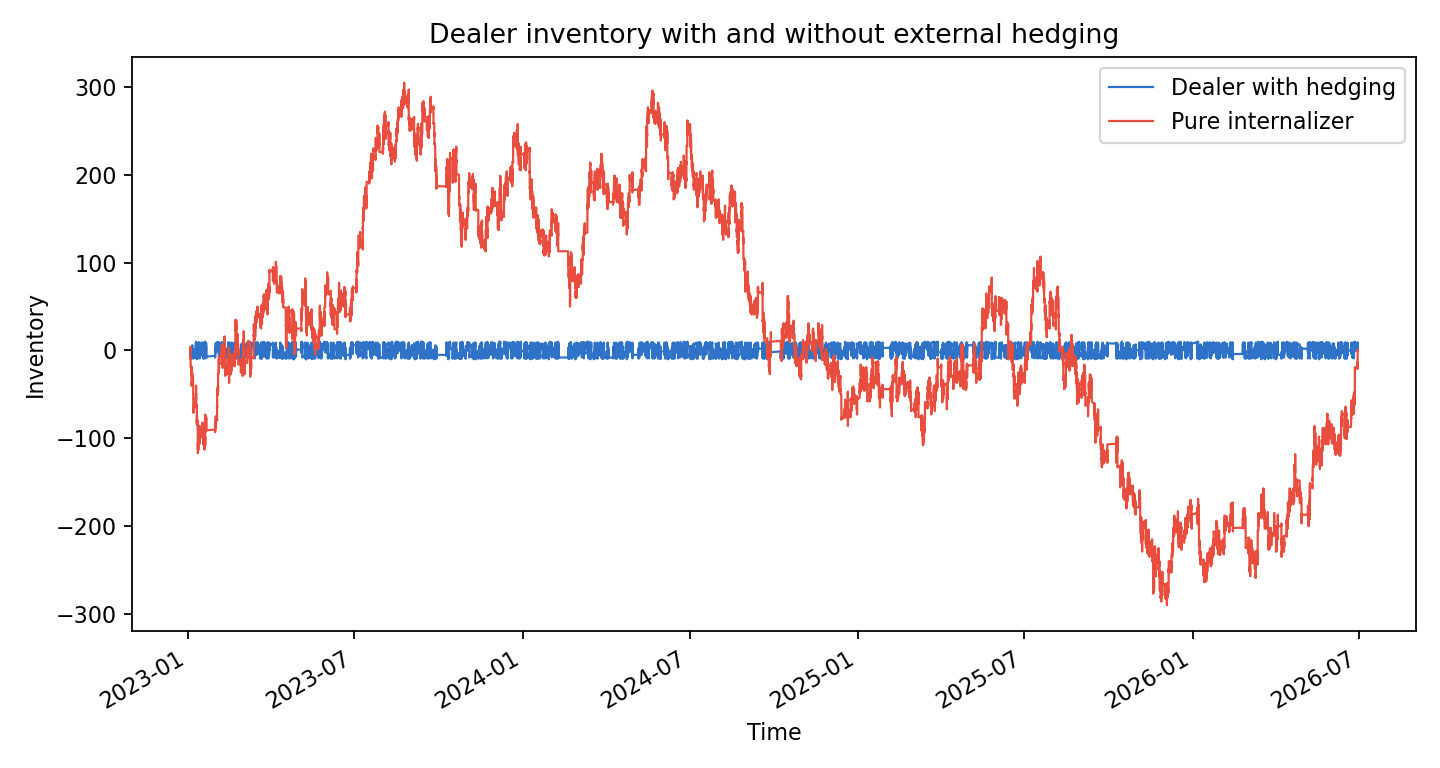
\includegraphics[width=.84\textwidth]{dealer_hedging_inventory.png}\caption{分钟代理中的dealer库存：外部对冲与纯内部化}\end{figure}
\begin{figure}[H]\centering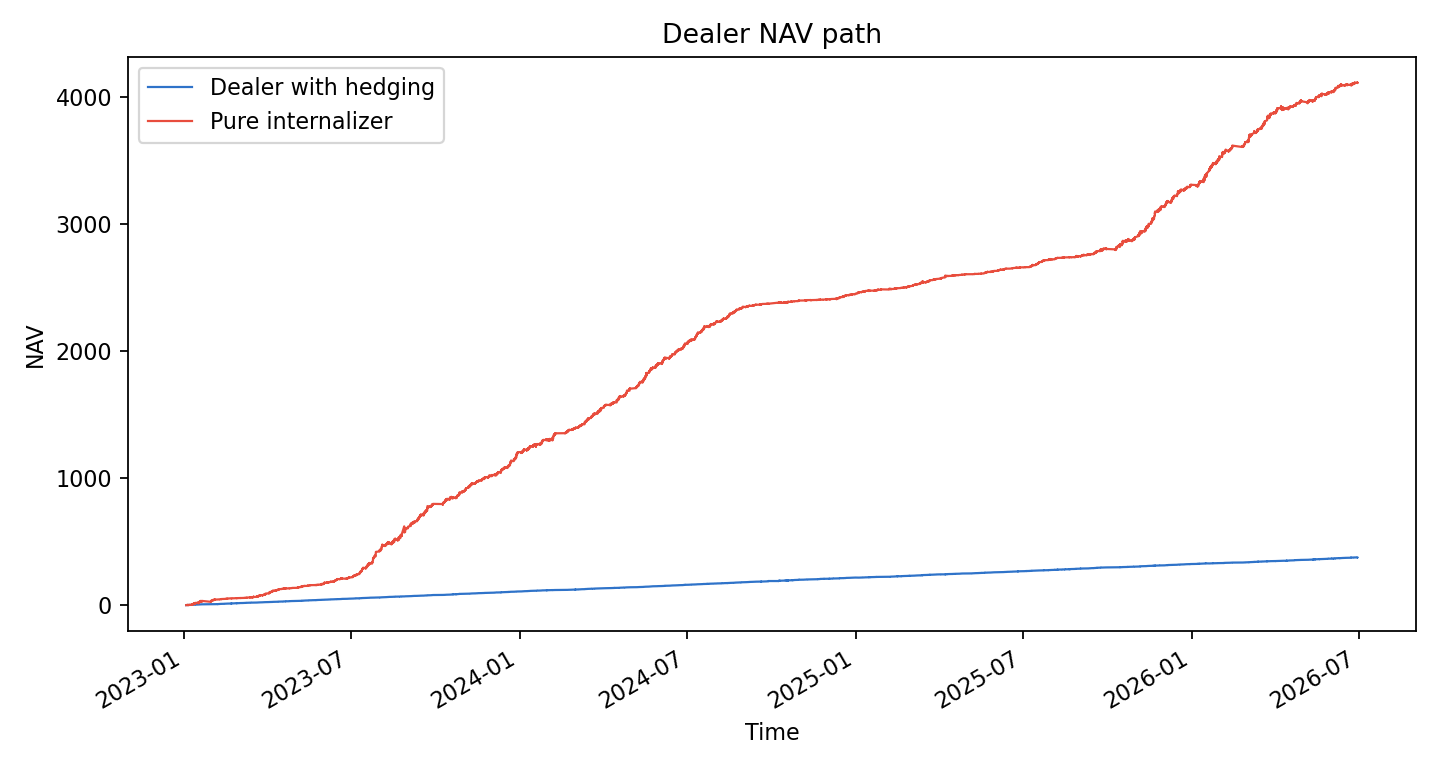
\includegraphics[width=.84\textwidth]{dealer_hedging_nav.png}\caption{分钟代理中的净值路径及风险收益交换}\end{figure}

\section{hftbacktest事件流与撮合设置}
框架轨道使用60秒、1毫秒步长的合成L2事件。初始中间价100、tick size为0.01，买卖各20档、每档12手。中间价以30\%概率移动一个tick，主动交易以55\%概率到达，数量1至4手。固定随机种子保证目标与基准面对完全相同的市场路径。

订单进场和回报延迟均为10毫秒，策略每50毫秒更新一次。队列采用risk-adverse模型，交易所采用完整一手成交，maker费率为$-2$ bp、taker费率为$7$ bp。所有主要报价为post-only限价单。若目标报价穿过对手价，系统退回一档，避免库存压力无意中变为主动吃单。

每次更新并非清空全部订单。价格仍符合目标的订单继续保留队列位置；偏离目标的订单先撤销，再提交新单。Recorder保存时间戳、价格、现金、费用、仓位与累计成交，权益定义为$E_t=B_t+q_tS_t-F_t$。这使延迟、撤单和队列进入统一状态机，而不是由自写循环假定即时成交。

\section{目标策略与基准}
纯internalizer在所有状态使用温和偏斜$0.22q$，所以它不是完全没有风险控制的弱基准。目标策略在$|q|\le4$时与基准完全相同；当$|q|>4$时进入风险紧迫状态。正库存下调报价中心，使卖单更积极、买单更保守；负库存反向。\texttt{hedge\_urgency\_events}记录进入紧迫状态的策略周期数，不能被解释为真实外部对冲成交数。

选择这种诚实标注，是因为当前只有一个合成交易场所。如果直接把同场所的主动成交称为inter-dealer hedge，会混淆订单簿去库存与跨场所对冲。未来应增加第二资产或第二场所，提交IOC或marketable limit order，并单独记录外部价差、手续费和冲击。

\section{框架结果与逐指标解释}
\begin{table}[H]\centering\caption{hftbacktest dealer机制结果}\begin{tabular}{lrrrrrr}\toprule
策略&最终PnL&权益std&库存均值&库存std&最大仓位&成交数\\\midrule
风险紧迫策略&1.959&1.996&0.072&2.602&7&1005\\
纯内部化&3.233&2.247&0.197&2.805&8&1037\\\bottomrule\end{tabular}\end{table}

目标策略触发80个风险紧迫周期。库存标准差下降7.2\%，最大绝对库存下降12.5\%，权益标准差下降11.1\%；代价是终端PnL下降39.4\%、成交数下降3.1\%。库存均值均接近零，但均值会因正负抵消，不能替代标准差与尾部仓位。结果方向与论文机制一致：越界后的积极去库存降低风险，却牺牲部分价差机会。

风险下降幅度小于A--S项目，因为两个dealer策略在大多数舒适区状态完全相同，只有80个周期发生分歧；而且当前仍依靠后续被动成交去库存，不能保证立即回到阈值内。完整主动对冲预计会更快压低仓位，但成本也会更清晰。

\section{阈值失败、调试与识别}
第一版阈值设为8，纯internalizer的最大绝对库存也恰好为8。代码条件是$|q|>8$，因此目标分支一次也没有执行，两个策略所有指标完全相同，紧迫事件为0。这不是模型验证成功，而是机制没有被样本触发。

把阈值收紧至4后，风险状态出现80次，结果才与基准分离。该过程说明回测必须检查状态覆盖，而不能只检查代码是否包含某个参数。更完整的下一版应保存每次进入/退出风险区的时间、连续停留长度、反向成交数和回归舒适区所需时间。

\section{外部对冲扩展设计}
真正的外部对冲数量可定义为
\[
h_t=-\operatorname{sign}(q_t)\min\{\eta(|q_t|-q^*),h_{\max}\}.
\]
客户市场作为资产0继续被动报价，外部市场作为资产1提交IOC订单。成本函数可写为$C(h)=c_1|h|+c_2h^2$，分别表示价差/手续费与非线性冲击。策略还必须跟踪在途订单，用$q+q_{pending}$而不是当前$q$计算新需求，防止延迟期间重复过度对冲。

评价指标需要新增客户价差收入、外部对冲成本、内部化比例、hedge turnover、风险区占比、库存95\%/99\%分位数和最大连续暴露时间。只有把收入和成本拆开，才能回答“风险下降是否值得”。

\section{稳健性与限制}
稳健性实验应首先对30至100个市场种子做成对比较，报告$\Delta$PnL与$\Delta$库存风险分布。其次比较阈值2、4、6、8，紧迫偏斜0.5至2.0，以及延迟1至100毫秒。市场状态需覆盖趋势、均值回复、高波动和单边客户流。若策略只在某一条路径或某一个阈值有效，不能形成一般结论。

当前结果不能证明真实dealer市场盈利：合成L2不是历史订单簿，分钟客户流是代理，紧迫报价不是实际跨场所对冲，maker返佣也不是A股费率。本文能够证明的是：论文核心状态机制已经进入专业订单状态机，并在机制确实触发后产生可识别的风险收益交换。

\section{代码结构与逐函数映射}
项目的理论函数位于\texttt{src/dealer\_model.py}。\texttt{DealerParams}集中保存半价差、库存偏斜、对冲阈值、外部化比例、冲击成本、客户成交概率和最大交易数量，避免参数散落在循环中。\texttt{quote\_adjustment}把库存转换为买卖深度：长库存扩大买单深度并缩小卖单深度，短库存相反；\texttt{hedge\_quantity}只在库存超过阈值后返回反向数量。单元测试验证长库存确实惩罚继续买入，并验证阈值内不对冲、阈值外对冲方向正确。

分钟入口\texttt{scripts/run\_research\_pipeline.py}负责按月请求或读取Tushare分钟数据，排序、去重并转换时间戳。\texttt{run\_strategy}以相同随机种子分别运行有对冲和纯内部化策略，保证客户流路径一致。每次客户成交后计算外部对冲数量，再以当前mid和冲击代理价格更新现金与库存，最后使用下一分钟close盯市。输出包括完整路径CSV、策略汇总CSV、运行元数据JSON和两张图。

hftbacktest入口则把论文机制映射到订单状态机。策略每次调用\texttt{hbt.elapse}推进事件时间，清理已失效订单，读取market depth与实际position，计算目标中心和半价差，然后遍历活动订单做reconcile。买卖订单编号分开，库存上限决定某一侧是否允许继续挂单。每次Record发生在订单处理后，使仓位、余额和费用能够对应同一策略周期。

\section{参数表与单位审计}
\begin{table}[H]\centering\caption{dealer项目主要参数、单位与作用}\begin{tabularx}{\textwidth}{lclX}\toprule
参数&数值&单位&作用\\\midrule
tick size&0.01&价格&离散报价网格\\
lot size&1&手&每笔做市订单数量\\
normal skew&0.22&tick/手&舒适区内温和库存偏斜\\
trigger&4&手&进入风险紧迫状态的严格阈值\\
urgent skew&1.35&tick/手&越界后的去库存强度\\
normal spread&3&tick&普通状态半价差\\
urgent spread&1&tick&风险状态半价差\\
max position&45&手&阻止继续增加极端库存\\
requote&50&毫秒&报价检查与更新周期\\
order latency&10/10&毫秒&进场/回报固定延迟\\
maker fee&-0.00002&比例&被动成交费用路径\\
\bottomrule\end{tabularx}\end{table}

参数审计不仅检查数值是否写入代码，还检查单位与触发。偏斜以tick/手表示，不能直接与分钟代理中的价格单位混用。阈值条件使用严格大于号，因此阈值8在最大仓位恰好8的路径上不会触发。硬上限45远高于实际最大仓位8，没有主导本次结果。maker负费率表示返佣，不能直接对应中国ETF费用，但目标和基准共享该设置，组内比较仍保持一致。

\section{PnL与风险的进一步分解}
当前权益变化可概念性拆为客户/做市价差收入、库存盯市、费用和未来外部对冲成本：
\[
\Delta E=\mathrm{SpreadCapture}+q\Delta S-\mathrm{Fees}-\mathrm{ImpactCost}.
\]
框架轨道尚未显式标记每笔成交属于价差还是库存盯市，因此final PnL较低不能直接归因于某一个成本项。风险紧迫策略收窄价差，可能降低单笔价差收入；更强偏斜也可能让部分订单远离市场、减少成交；与此同时仓位下降会减少$q\Delta S$波动。下一版应在成交回报时保存成交价、当时mid和延后mid，分别计算实现价差与markout。

权益标准差下降11.1\%比库存标准差下降7.2\%更大，可能说明目标不仅降低仓位幅度，也改变了仓位与价格变化的共同方向。要验证这一点，可以计算库存与未来价格变化的协方差，并按风险状态分组。最大仓位只下降一手，但风险状态持续时间可能明显缩短；因此还需报告库存超过4、6、8的时间占比和连续暴露长度。

\section{多路径稳健性实验矩阵}
第一组实验固定策略参数，只改变市场随机种子。至少运行50条路径，并对每条路径成对计算目标减基准的PnL、库存标准差、权益标准差和最大仓位。报告均值、中位数、5\%与95\%分位数，以及目标风险更低的路径占比。成对差值比两组独立均值更能利用共同市场路径控制噪声。

第二组改变市场状态。趋势路径检验长期单边客户流下的库存积累；均值回复路径检验过早对冲是否损失自然回归收益；高波动路径检验风险区是否更频繁触发；低流动性路径检验紧迫报价是否仍能成交。第三组改变执行假设，包括延迟1、10、50、100毫秒，部分成交开关，不同队列模型和maker/taker费用。

第四组做参数网格。阈值$q^*$取2、4、6、8；紧迫偏斜取0.5、1.0、1.35、2.0；紧迫半价差取1、2、3 tick。不能从全网格中只挑最高PnL，而应画风险收益前沿：横轴库存或权益风险，纵轴PnL，标出每个参数组合。若某组合风险更高且收益更低，则被另一组合严格支配。

\section{真实Level2与双场所数据需求}
真实dealer复现至少需要两类数据。客户侧需要RFQ时间、方向、数量、dealer报价、是否成交和客户类别；外部侧需要订单簿、逐笔成交、主动方向、订单延迟与实际执行价。若只能获得交易所Level2而没有RFQ，仍可研究“交易所做市+外部对冲”，但不能声称完整复现dealer客户市场。

数据清洗需检查时间戳时区、交易日边界、重复消息、序列号缺口、交叉盘口和快照恢复。两场所价格还需统一合约乘数、tick、lot和费用。回放时客户成交应改变dealer库存，外部对冲订单必须经过另一个场所的队列和延迟，不能在同一循环中按mid无条件成交。

\section{复现命令与验收清单}
分钟代理通过\texttt{python scripts/run\_research\_pipeline.py}运行；框架轨道通过\texttt{python scripts/run\_hftbacktest.py}运行；单元测试使用\texttt{python -m pytest -q}。每次结果验收应确认：数据起止时间与观测数存在；两策略使用相同随机种子；summary中两组指标非空；紧迫事件大于零；目标与基准结果不完全相同；图形与CSV更新时间一致。

报告编译使用XeLaTeX两次，以更新目录和交叉引用。正式Git提交只保留\texttt{report.tex}、\texttt{report.pdf}和必要图形，不保留aux、log、out、toc等中间文件。结果JSON应包含synthetic L2边界，避免以后只看到文件名就误认为真实历史回放。

\section{指标公式与报告口径附录}
库存均值$\bar q=N^{-1}\sum_t q_t$只反映方向偏置；库存标准差$\sigma_q=[N^{-1}\sum_t(q_t-\bar q)^2]^{1/2}$反映典型波动；最大绝对库存$\max_t|q_t|$反映最坏资本占用。权益标准差使用所有Recorder时点而不是逐期收益，表示路径离散程度。成交数是累计完整成交，不包含撤单和未成交报价。紧迫事件是处于风险状态的策略周期，不是订单或成交数量。

为了便于比较，风险下降率定义为$(R_{base}-R_{target})/R_{base}$，PnL变化率定义为$(P_{target}-P_{base})/|P_{base}|$。本次库存标准差下降7.2\%、权益标准差下降11.1\%，PnL下降39.4\%。由于只有一条路径，这些百分比没有置信区间，不能写成总体参数。多路径版本应先对每条路径计算差值，再对差值汇总，而不是先平均两个策略后相减。

最大回撤尚未列为主要指标，因为初始权益为零、短路径且权益包含库存盯市，百分比回撤容易失真。未来可报告绝对回撤、尾部库存ES、风险区连续时长和单位风险下降成本。dealer项目尤其应报告每减少一单位库存标准差所付出的对冲成本，才能比较不同阈值。

\section{课堂汇报中的关键问答}
若被问“为什么风险策略利润更低还值得研究”，应回答论文目标不是无成本增收，而是用可控成本降低库存尾部和资本占用。若被问“这是否是真实外部对冲”，必须说明当前hft轨道是风险紧迫报价，分钟轨道才有显式数量外部化代理，两者都不是实际inter-dealer逐笔回放。

若被问“阈值4是否为了让结果好看”，应展示阈值8时紧迫事件为0、两组结果完全相同的诊断。阈值4的作用是保证机制在样本内被识别，并不保证PnL改善；事实上目标PnL更低，说明没有为了美化收益调参。若被问“下一步最重要的改进”，答案是第二场所主动对冲与真实Level2，而不是继续改变图表样式。

若被问“为什么不使用Hummingbot”，可以说明hftbacktest更适合历史事件回放、队列和延迟；Hummingbot更适合连接器、纸面交易和跨场所运行。真正的dealer双场所扩展可以先在hftbacktest验证历史执行，再用Hummingbot验证实时连接器行为，两者角色不同。

\section{结论}
本项目把dealer库存内部化与外部风险处置从自写分钟循环推进到hftbacktest统一撮合环境。目标策略降低库存和权益波动，但终端PnL较低，体现对冲并非免费。阈值未触发的初始失败进一步说明，策略存在、策略运行和策略有效是三个不同层次。下一阶段最重要的工作是加入第二场所的主动对冲、真实Level2样本和多路径稳健性，而不是继续寻找单一路径上更漂亮的收益。

\begin{thebibliography}{9}
\bibitem{bbg} A. Barzykin, P. Bergault, and O. Guéant. \emph{Algorithmic market making in dealer markets with hedging and market impact}. 2021.
\bibitem{as} M. Avellaneda and S. Stoikov. \emph{High-frequency trading in a limit order book}. Quantitative Finance, 2008.
\bibitem{hft} \texttt{hftbacktest} documentation, version 2.4.
\end{thebibliography}\end{document}
